\usetikzlibrary{spy}
\definecolor{setpoint}{RGB}{54,54,54}
\definecolor{limitpoint}{RGB}{193,102,53}
\definecolor{curvepoint}{RGB}{201, 152, 125}

\begin{center}
\begin{tikzpicture}[
  every node/.style={inner sep=0pt},
  spy using outlines={circle, magnification=5, size=2.6cm, connect spies},
]

  \def\xscale{0.6}
  \def\yscale{6}
  \def\yshift{0.43}
  \def\ymaxband{6.07}

  % --- Horizontal shaded bands, fading from white into limitpoint's color near p ---
  \foreach \y [remember=\y as \yprev (initially \ymaxband)] in {5.82,5.57,...,0}{
    \pgfmathsetmacro{\xA}{(\yscale/(\yprev+\yshift))*\xscale}
    \pgfmathsetmacro{\xB}{(\yscale/(\y+\yshift))*\xscale}
    \pgfmathsetmacro{\yavg}{(\yprev+\y)/2}
    \pgfmathsetmacro{\op}{0.4*(1-\yavg/\ymaxband)}
    \fill[limitpoint, opacity=\op]
      (\xA,\yprev) -- (10.5,\yprev) -- (10.5,\y) -- (\xB,\y) -- cycle;
  }

  % axes
  \draw[thick, setpoint, ->] (0.5,0) -- (0.5,6.5);
  \draw[thick, setpoint, ->] (0.5,0) -- (10.2,0);

  % label for the sequence
  \node[setpoint, font=\small] at (2.5,2) {$f(n) = \dfrac{1}{n}$};

  % curve, drawn on top of the shading
  \draw[curvepoint, thick, domain=0.923:12.5, samples=100, smooth]
    plot (\x*\xscale, {(\yscale/\x)-\yshift});

  % vertical number line
  \draw[thick, setpoint, ->] (10.5,-0.3) -- (10.5,6.8);

  \foreach \n in {1,2,3,4,5,6,7,8,9,10,11,12,13,14}{
    \pgfmathsetmacro{\ypos}{\yscale/\n}
    \filldraw[setpoint] (10.5,\ypos) circle (1.8pt);
  }

  \foreach \n in {18,25,35,50,70,100,150,250}{
    \pgfmathsetmacro{\ypos}{\yscale/\n}
    \filldraw[setpoint] (10.5,\ypos) circle (1.5pt);
  }

  \filldraw[limitpoint] (10.5,0) circle (2.6pt);
  \node[limitpoint, right, font=\small] at (10.7,0) {$p$};

  \spy [limitpoint, magnification=5, size=2.6cm] on (10.5,0.08) in node at (13.2,3.2);

\end{tikzpicture}
\end{center}
